%% General definitions
\documentclass{article} %% Determines the general format.
\usepackage{a4wide} %% paper size: A4.
\usepackage[utf8]{inputenc} %% This file is written in UTF-8.
%% Some editors on Windows cannot save files in UTF-8.
%% If there is a problem with special characters not showing up
%% correctly, try switching "utf8" to "latin1" (ISO 8859-1).
\usepackage[T1]{fontenc} %% Format of hte resulting PDF file.
\usepackage{fancyhdr} %% Package to create a header on each page.
\usepackage{lastpage} %% Used for "Page X of Y" in the header.
											%% For this to work, you have to call pdflatex twice.
\usepackage{enumerate} %% Used to change the style of enumerations (see below).

\usepackage{amssymb} %% Definitions for math symbols.
\usepackage{amsmath} %% Definitions for math symbols.
\usepackage{amsthm}
\usepackage{braket}
\usepackage{graphicx}
\usepackage{float}

\usepackage{tikz}  %% Pagacke to create graphics (graphs, automata, etc.)
\usetikzlibrary{automata} %% Tikz library to draw automata
\usetikzlibrary{arrows}   %% Tikz library for nicer arrow heads


%% Left side of header
\lhead{\course\\\semester\\Exercise \homeworkNumber}
%% Right side of header
\rhead{\authorname\\Page \thepage\ of \pageref{LastPage}}
%% Height of header
\usepackage[headheight=36pt]{geometry}
%% Page style that uses the header
\pagestyle{fancy}

\newcommand{\authorname}{Nico Bachmann\\Ruben Hutter}
\newcommand{\semester}{Spring semester 2023}
\newcommand{\course}{Theory of Computer Science}
\newcommand{\homeworkNumber}{3}


\begin{document}

\section*{Exercise \homeworkNumber.1}
\begin{enumerate}[(a)]
	\item
	A possible derivation of the word "abaabaaba" is:
	$$
	1 \; (aSa) \to 2 \; (abSba) \to 1 \; (abaSaba) \to 1 \; (abaaSaaba) \to 4 \; (abaabaaba)
	$$
	
	\item
	$\mathcal{L}(G)$ is the definition of a Palindrome. The word can always be read either forward or
	backward and you get the same result.
	
	\item
	The Grammar that represents a representation of binary trees is:
	$$
	G = \left \langle \set{S}, \; \set{[, \circ, \square, ]}, \; R, \; S \right \rangle
	$$
	with R:
	\begin{enumerate}[1)]
		\item
		$S \to \square$
		
		\item
		$S \to [S \circ S]$
		
	\end{enumerate}
	
\end{enumerate}

\section*{Exercise \homeworkNumber.2}
\begin{enumerate}[(a)]
	\item
	The grammar $G_1 = \left \langle \set{S, X, Y}, \set{a, b}, R_1, S \right \rangle$ is of type-0
	because there is rule $S \to \epsilon$ and rule $S \to aS$ which violates the special case, where $S$
	never occurs on the right-hand side if $S$ also maps to the empty word.

	\item
	The grammar $G_2 = \left \langle \set{S, X, Y}, \set{a, b}, R_2, S \right \rangle$ is of type-1, and
	so also of type-0, because $baX \to baaX$ is context-sensitive. The other rules are of type-2 or
	type-3.

\end{enumerate}

\section*{Exercise \homeworkNumber.3}
The regular grammar for the given DFA is:
$$
G = \left \langle \set{S, U, V}, \; \set{a, b, c}, \; R, \; S \right \rangle
$$
with rules R as follows:
\begin{center}
	\begin{tabular}{ c c c }
 	$S \to aU$ & $S \to bV$ & $S \to c$ \\ 
 	$U \to aU$ & $U \to cS$ & $U \to c$ \\  
 	$V \to bV$ & $V \to cS$ & $V \to c$    
	\end{tabular}
\end{center}

\clearpage

\section*{Exercise \homeworkNumber.4}
\begin{figure}[h]
		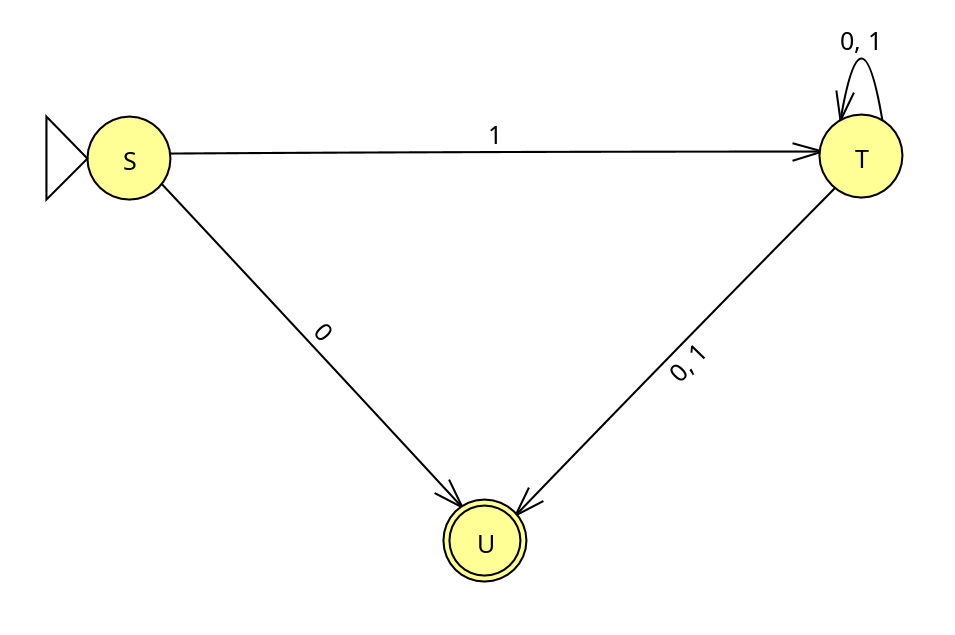
\includegraphics[width=\linewidth]{ex4.png}
		\centering
		\caption{NFA for $G$}
\end{figure}

\section*{Exercise \homeworkNumber.5}
\subsection*{Fist step}
We find the complement of $G_2$ by inverting the corresponding DFA.

\subsection*{Second step}
Given the equivalence problem: $A = B \quad \text{iff} \quad (A \cap B^c) \cup (A^c \cap B) = \emptyset$
which applies in both directions, we can extrapolate only the $(A \cap B^c)$ part in order to obtain $A \subseteq B \quad \text{iff} \quad (A \cap B^c) = \emptyset$. Because regular languages are closed under intersection and complement, and we know algorithms for these operations.

\subsection*{Third step}
Decide if $(A \cap B^c)$ is $\emptyset$ by using the algorithm for the emptiness problem $P_\emptyset$.

\end{document}
